\chapter{mdsearch Documentation}
\label{chap:mdsearch}
\centerline{\rule{149mm}{.02in}}
\vspace{2cm}

mdsearch is a small C++ library that implements a subset of the index structures discussed in this report. The library is available to download on an online Git repository \footnote{\url{https://github.com/DonaldWhyte/mdsearch}}. This library makes heavy use of template metaprogramming and inline functions to boost performance. As such, it is a header-only library. Each implemented index structure can be used by simply including its corresponding header file.

Currently, the following index structures have been implemented:
\begin{itemize}
	\item \textbf{Pyramid Tree} -- see Section \ref{sec:pyramid-tree-detail} for more information
	\item \textbf{$kd$-Tree} -- see Section \ref{sec:kd-tree-detail} for more information
	\item \textbf{Bucket Hash Table} -- see Section \ref{sec:bucket-hash-table} for more information
	\item \textbf{Multigrid} -- see Section \ref{sec:multigrid} for more information
\end{itemize}

\section{Dependencies}

mdsearch requires the following header-only Boost libraries
\begin{itemize}
	\item Boost.Unordered
	\item Boost.Functional/Hash
	\item Boost.Lexical\_Cast
\end{itemize}

\section{API}

Each index structure is represented as a class, which implements the three operations evaluated in the project. Therefore, each index structure class has the following methods:
\begin{itemize}
	\item \texttt{bool insert(point)} -- inserts unique point into the structure. Returns true if point insertion was successful and false if point is already being stored and has not been inserted.
	\item \texttt{bool remove(point)} -- deletes point from structure. Returns true if the point was found and deleted successful and false if the point was not found.
	\item \texttt{bool query(point)} -- returns true if point is being stored in structure and false otherwise.
\end{itemize}

Table \ref{tab:library-classes} describes the role of each class in the library. Figure \ref{fig:library-class-diagram} illustrates the inheritance and dependencies between these classes using a UML class diagram.

\begin{table}[H]
	\centering
	\begin{tabular}{|p{4.25cm}|p{9.5cm}|}
		\hline
		\textbf{Data Type} & \textbf{Description} \\
		\hline
		\texttt{Real} & Type of individual coordinate of point \\
		\texttt{RealList} & Re-sizeable array of \texttt{Real}s \\
		\texttt{HashType} & Type of discrete hash value used by hash-based structures \\
		\texttt{Point<D>} & Point with D dimensions \\
		\texttt{Boundary<D>} & Boundary in D-dimensional space \\
		\texttt{Dataset<D>} & Dataset containing D-dimension points, which can load points from files and compute the minimum bounding region containing every point \\
		\texttt{KDTree<D>} & $kd$-tree for D-dimensional space \\
		\texttt{Multigrid<D>} & Multigrid for D-dimensional space \\
		\texttt{HashStructure<D>} & Abstract class for hash-based structures, which follows the Bucket Pseudo-Pyramid Tree structure described in Section \ref{sec:iteration1} closely \\
		\texttt{PyramidTree<D>} & Pyramid Tree for D-dimensional space \\
		\texttt{BucketHashTable<D>} & Bucket Hash Table for D-dimensional space \\
		\hline
	\end{tabular}
	\caption{Descriptions of Each Type in mdsearch Library}
	\label{tab:library-classes}
\end{table}

\begin{figure}[H]
	\centering
	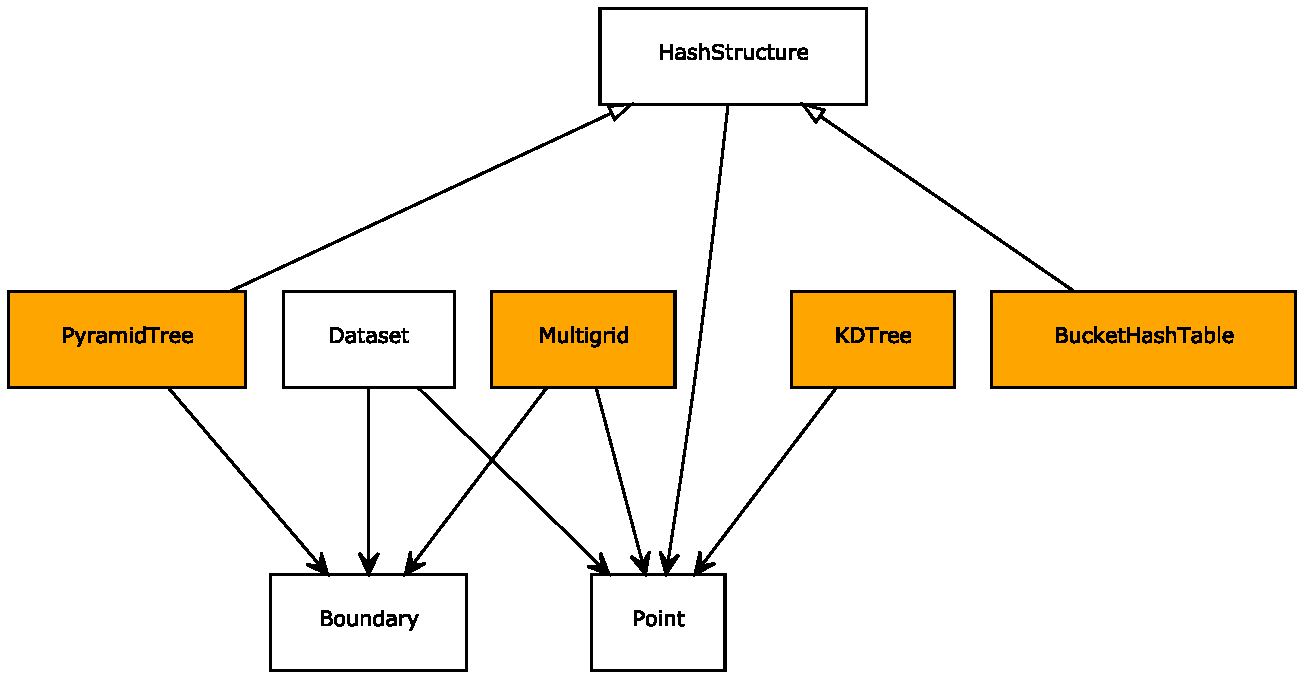
\includegraphics[scale=0.6]{figures/mdsearch_classes_uml.pdf}
	\caption{UML Class Diagram of mdsearch Library. Coloured Boxes Represent Index Structures.}
	\label{fig:library-class-diagram} 
\end{figure}

\section{Examples}

The library comes with a program that generates random points and performs a set of correctness tests on each index structure. This program is contained within the \texttt{test\_structures.cpp} file and as such ,